%%%%%%%%%%%%%%%%%%%%%%%%%%%%%%%%%%%%%%%%%%%%%%%%%%%%%%%%%%%%%%%%%%%%%%%%%%%%%
%
% qucomp.tex --- main file of the dissertation
%
% Originally written 2004 (Bilgi University, supervisor Bulent Ozel).
% Modernised 2026 for current TeX Live / pdflatex; chapters revised
% per the corrigendum that accompanies this revision.
%
%%%%%%%%%%%%%%%%%%%%%%%%%%%%%%%%%%%%%%%%%%%%%%%%%%%%%%%%%%%%%%%%%%%%%%%%%%%%%
\documentclass[12pt,letterpaper]{article}

% --- core packages ---------------------------------------------------------
\usepackage[utf8]{inputenc}
\usepackage{cmap}                       % proper Unicode mappings in PDF
                                        % (must be loaded before fontenc)
\usepackage[T1]{fontenc}
\usepackage{lmodern}                    % Latin Modern (Type 1, ligatures
                                        % extract as real text)
\usepackage[letterpaper,margin=1in]{geometry}
\usepackage{graphicx}
\usepackage{latexsym}
\usepackage{array}
\usepackage{tabularx}
\usepackage{lscape}
\usepackage{amsmath,amssymb,amsfonts}
\usepackage{rotating}
\usepackage{fancyhdr}
\usepackage{setspace}
\usepackage{listings}
\usepackage{xcolor}
\usepackage{hyperref}

% --- spacing ---------------------------------------------------------------
\onehalfspacing
\setlength{\emergencystretch}{3em}      % gives TeX extra slack on paragraphs
                                        % containing long unbreakable \texttt
                                        % tokens like file paths
\hbadness=2000                           % suppress tiny underfull warnings
                                        % (overfull boxes still warned)

% --- shorthands ------------------------------------------------------------
\def\ma#1{{\tt #1}}
\def\tv#1{{\scriptstyle(#1)}}

% Dirac notation
\def\bra#1{\mathinner{\langle{#1}|}}
\def\ket#1{\mathinner{|{#1}\rangle}}
\newcommand{\braket}[2]{\langle #1|#2\rangle}
\def\Bra#1{\left<#1\right|}
\def\Ket#1{\left|#1\right>}

% Title
\newcommand{\disstitle}{Quantum Computation:\\Implementation of Quantum Gates on Linux Clusters}

% --- page style ------------------------------------------------------------
\setlength{\headheight}{14.5pt}         % silence fancyhdr warning
\pagestyle{fancy}
\newenvironment{itemizeeng}{\begin{itemize}\itemsep-0.8ex minus0.1ex}{\end{itemize}}
\renewcommand{\sectionmark}[1]{\markright{\thesection.\ #1}}
\lhead{}\chead{}\rhead{}
\lfoot{}\cfoot{}\rfoot{}
\renewcommand{\headrulewidth}{0.0pt}
\renewcommand{\thefootnote}{\fnsymbol{footnote}}

% --- bibliography ----------------------------------------------------------
\bibliographystyle{plain}

% --- math ------------------------------------------------------------------
\newtheorem{definition}{Definition}
\newtheorem{theorem}{Theorem}

% Number equations per-section so hyperref destination IDs stay unique
% (otherwise every section's \setcounter{equation}{0} creates "equation.1"
%  collisions in the PDF).
\numberwithin{equation}{section}
\renewcommand{\theHequation}{\thesection.\arabic{equation}}

% --- listings (for C code samples in revised chapters) ---------------------
\lstdefinestyle{cstyle}{
    language=C,
    basicstyle=\ttfamily\small,
    keywordstyle=\color{blue!70!black}\bfseries,
    commentstyle=\color{green!40!black},
    stringstyle=\color{red!70!black},
    showstringspaces=false,
    breaklines=true,
    numbers=left,
    numberstyle=\tiny\color{gray},
    frame=single,
    framerule=0.4pt,
    rulecolor=\color{gray!30},
    xleftmargin=2em,
    tabsize=4,
    captionpos=b
}
\lstset{style=cstyle}

% --- hyperref colours ------------------------------------------------------
\hypersetup{
    colorlinks=true,
    linkcolor=blue!50!black,
    citecolor=blue!50!black,
    urlcolor=blue!60!black,
    plainpages=false,                    % use formatted page label, not raw int
    hypertexnames=false,                 % auto-generate unique anchor names
                                         % (prevents page.1 collisions when
                                         %  \pagenumbering is reset)
    pdftitle={Quantum Computation: Implementation of Quantum Gates on Linux Clusters},
    pdfauthor={Arda Karaduman}
}

\makeindex
%%%%%%%%%%%%%%%%%%%%%%%%%%%%%%%%%%%%%%%%%%%%%%%%%%%%%%%%%%%%%%%%%%%%%%%%%%%%%

\begin{document}
\begin{titlepage}
\vspace*{\fill}
\begin{center}
\Large
\.{I}STANBUL B\.{I}LG\.{I} UNIVERSITY\\
FACULTY of\\
SCIENCE AND LETTERS\\

\vspace{3\bigskipamount}

\large
{\em \disstitle}

\vspace{3\bigskipamount}

SUBMITTED By\\
Arda Karaduman

\vspace{2\bigskipamount}

In Partial Fulfillment of the Requirements for the Degree of\\
Bachelor of Science in Computer Science\\

\vspace{2\bigskipamount}

\today

\vspace{3\bigskipamount}

APPROVED By\\

\begin{tabular*}{\textwidth}{@{\extracolsep{\fill}}cc}
Chris Stephenson	&	B\"{u}lent \"{O}zel \\
Head of Department	&	Dissertation Supervisor\\
\end{tabular*}

\end{center}
\vspace*{\fill}\par
\end{titlepage}

\pagenumbering{roman}
\doublespacing
\newpage
\vspace*{\fill}
\begin{center}
{\bf Foreword}
\end{center}
\addcontentsline{toc}{section}{Foreword}

My original dissertation thesis in 2004 was incomplete. This has been bugging me for a while, so I decided to revamp it using AI.

I stayed true to the state of facts as of 2004, filled in the missing algorithms, sketched the implementation strategy that the parallel simulator should have used, and made the build itself easier to execute in 2026 --- except in Section~\ref{sec:parallel}, where the implementation strategy is informed by what the simulator community has converged on since.

\vspace{1\bigskipamount}

\hfill --- Arda Karaduman, May 21, 2026
\vspace*{\fill}

\newpage

\rhead{\bfseries \thepage}
\vspace*{\fill}
\begin{center}
{\bf Abstract}
\end{center}
\addcontentsline{toc}{section}{Abstract}
This thesis gives an introduction to {\tt Quantum Computation} and discusses implementation strategies for a {\tt Quantum Computer} simulator on a distributed system. Research into {\tt Quantum Computers} has expanded rapidly since Peter Shor showed that integer factorisation --- believed to be classically intractable --- admits a polynomial-time quantum algorithm; further quantum algorithms have since been discovered that outperform their classical counterparts on a range of problems. Physical realisation of {\tt Quantum Computers} remains difficult, and machines built to date are limited in size and noisy in operation; as a result, much of the research into {\tt Quantum Computation} algorithms makes use of simulators running on classical hardware. The fundamental difference between classical and quantum computation makes such simulation inherently expensive: the state vector grows exponentially in the number of qubits. This thesis examines the strategies available for simulating a {\tt Quantum Computer} on a parallel {\tt Linux} cluster, identifies the central scaling pitfall of dense-matrix approaches, and presents the in-place sparse-gate strategy that scalable simulators must adopt instead. It then applies that strategy to the three canonical quantum algorithms: the {\tt Quantum Fourier Transform}, Grover's unstructured search, and Shor's integer factorisation.
\vspace*{\fill}

\newpage

\addcontentsline{toc}{section}{Table of Contents}
\tableofcontents

\newpage
\addcontentsline{toc}{section}{List of Figures}
\listoffigures

\newpage
\pagenumbering{arabic}
\setcounter{equation}{0}
\section{Introduction}


Since the first computers, the trend has been to miniaturize these machines in order to increase their efficiency and convenience. But, clearly nature has limits to this miniaturization process. It was Benioff \cite{cps80} who proposed that the ultimate limit of miniaturization would be a quantum mechanical system. However, soon after Deutsch \cite{qtct85} showed that the only benefits of a quantum computer was not it's size and energy savings, a totally new way of computation was possible which made use of the entangled quantum particles and quantum parallelization. Following this, Shor \cite{ptafpf94} discovered a polynomial time prime factorization algorithm for a quantum computer which garnered a great interest into quantum computation. Together with Grover's algorithm for the fast searching of an unsorted database \cite{fqma96}, Shor's algorithm provided the motivation for the scientists to research the possibilities of realization of a quantum computing device.

Despite the rapid progress on the theory of quantum computation, the experiments for physical implementation of a quantum computer faced major challenges. Although very basic quantum computing devices have been accomplished using different techniques, realization of a useful quantum computer in the near future seems impossible.

Because of this reason quantum computer simulation by classical computers became a popular topic. Many libraries \footnote{Lib Quantum (\emph{http://www.enyo.de/libquantum/})} and standalone applications have been developed for this purpose, some of them free, \footnote {Jaquzzi (\emph{http://www.eng.buffalo.edu/~phygons/jaQuzzi/jaQuzzi.html}) } \footnote {Qudit (\emph{http://www.compsoc.nuigalway.ie/~damo642/QuantumSimulator/QuantumSimulator/QuantumQuditSimulator.htm})} some of them proprietary \footnote{Senko's simulator (\emph{http://www.senko-corp.co.jp/qcs/qcp/qcpe.html})},and some languages have been developed \footnote { QCL (\emph{http://tph.tuwien.ac.at/~oemer/qcl.html})} \footnote {Q language (\emph{http://sra.itc.it/people/serafini/qlang/})}. Because computation complexity increases exponentially with the number of qubits simulated, these attempts suffer great performance problems. To overcome these problems, this thesis discusses a method for quantum computer simulation on a distributed system. A similar approach has been tried by B. Oemer and Glendinning \cite{pgsq03}.

\setcounter{equation}{0}
\section{History of Quantum Computation}


In 1982, acting independently, Richard Feynman and Paul Benioff has claimed that quantum computing could be possible. Simulating quantum systems on classical computers requires an exponentially large amount of time. Feynman's first motivation was these kind of operations, he proposed that a quantum system could simulate other quantum systems more efficiently \cite{spwc82}. Benioff's motivation was rather continuing the the trend of miniaturization in computer industry \cite{cps80}. As circuits continue to shrink they will eventually reach atomic level, and quantum mechanical effects would become a major limiting factor. So the only feasible solution was to construct a computer which would make use of quantum mechanical effects.

In 1985 David Deutsch published a paper \cite{qtct85} which proposed a quantum Turing machine, which made use of a before unnoticed property of quantum computers. Though severely underrated at its time, Deutsch's paper would later be considered a landmark in quantum computation theory. In his paper, Deutsch showed that it is possible to perform some tasks on quantum computers much more efficiently than classical computers. Deutsch's idea was to make use of a phenomenon which is known as quantum superposition. An isolated electron, if placed in a superposition, can travel along many different paths through a circuit. If the memory could be placed in a quantum superposition before applying the algorithm, it could be in multiple states simultaneously. So just one run-through the algorithm would calculate all computational paths simultaneously. This idea (Which was to be called \emph{quantum parallelism}) would be the foundation of all quantum algorithms.

The examples in Deutsch's paper were of limited use and due to their probabilistic nature, should be run several times to ensure the correct outcome. But these early hints in the field of quantum computation theory stirred the imaginations of many scientists, and about 10 years later Peter Shor of AT\&T labs came up with a factorization algorithm for quantum computers.

In 1994 Peter Shor of AT\&T developed a quantum computer algorithm for factorization \cite{ptafpf94} that is exponentially faster than any known classical algorithm. This discovery triggered a massive interest in quantum computation, because factorization is very hard to do classically, and all best known classical algorithms are super-polynomial. Factorization is known to be in the NP (Non-Deterministic Polynomial) complexity class, but it was believed that it was not in the P (Deterministic Polynomial) class and therefore thought to be intractably difficult on classical computers. These difficulties have been the basis of many modern crypto systems - including the widely used RSA (the Rivest-Shamir-Adleman protocol), which usually rely on the difficulty of factoring a very large number, which is the product of two prime numbers (secret keys). With Shor's algorithm, it has been shown that it is possible to factorize very large numbers with quantum computers, which would shake the security of known key exchange methods.

Only two years later Lov Grover of bell labs invented a quantum algorithm for fast searching of a database \cite{fqma96}. Although Grover's algorithm gives only a quadratic speed up over the best possible classical algorithm, the fact that searching forms the basis of many other algorithms, and the possibility to plugged in Grover's algorithm to existing algorithms to immediately increase their efficiency, increased the importance of Grover's discovery.

These algorithms show the capabilities of a quantum computer, and the main motivation behind the research into quantum computation. It is logical to expect even more powerful algorithms to be discovered in the near future. However, an implementation of a quantum computer which would be capable of convenient applications seems far away. Currently, quantum computers can operate only on a few qubits, and under extreme environmental conditions.





\setcounter{equation}{0}
\section{ Models of Computation}

Classical computers can be modeled by a Turing machine. A \emph{Turing Machine} is an abstract model of computation comprised of an infinitely long sequential tape, a read/write head, a set of symbols, and a set of rules for reading / writing and moving the head based on the symbol under it. These rules are called \emph{functions}, and the symbol under the head is called the \emph{state}. The machine moves from one state to another by executing a matching transition function. If no transition function matches, the machine halts.

The \emph{Church--Turing Thesis} \cite{ct36, tt36} says the following: a Turing machine can compute any function computable by a reasonable physical device. Programming languages can be translated into Turing machines and vice versa. Thus, the computation of any reasonable function can be expressed by a programming language.

The \emph{extended} (or \emph{strong}) Church--Turing thesis goes further than this and asserts that a probabilistic Turing machine can simulate any physical device with at most polynomial overhead. This is not a statement made by Church or Turing in their 1936 papers; it is a later thesis about the resources required for simulation. A \emph{probabilistic Turing Machine} can select among a set of transition functions with varying probability, instead of just one. In the following example, real numbers preceding a state indicate the probability of transitioning to that state.

\[ \begin{array}{ccccccc}
\ket{0} & \rightarrow & 0.5\ket{1} & + & 0.5\ket{2} \\
\ket{1} & \rightarrow & 0.2\ket{0} & + & 0.8\ket{1} \\
\ket{2} & \rightarrow & 0.4\ket{0} & + & 0.3\ket{2} & + & 0.3\ket{3} \\
\ket{3} & \rightarrow & 0.3\ket{0} & + & 0.7\ket{2} \end{array}\] 

Such machines can produce solutions with a negligible probability of error, which would be non computable if no error was tolerated. Probabilistic computation with negligible error is important for quantum computation.


\setcounter{equation}{0}
\section{Physical Background}

Quantum mechanics is a branch of physics which models the behavior of energy and matter at atomic and subatomic scales. Its name comes from \emph{quanta}\footnote{the discrete packets of energy proposed by Max Planck in 1900}.

Rather than enumerate informal ``theories'' of quantum mechanics, the cleanest way to present the subject is through its four postulates. Every result we use in this thesis --- superposition, entanglement, the reversibility of computation, measurement statistics --- is a consequence of these four statements and not an additional independent principle.

\subsection{The four postulates}

\paragraph{Postulate 1 (State space).} The state of an isolated quantum system is a unit vector in a complex Hilbert space $\mathcal{H}$. For a single qubit, $\mathcal{H} = \mathbb{C}^2$, and the state is
\begin{equation}
\ket{\psi} = \alpha\ket{0} + \beta\ket{1}, \qquad |\alpha|^2 + |\beta|^2 = 1.
\end{equation}
Two states that differ only by a global phase $e^{i\theta}$ are physically indistinguishable.

\paragraph{Postulate 2 (Evolution).} The evolution of a closed quantum system is unitary. A discrete time step is described by a unitary operator $U$ acting on the state:
\begin{equation}
\ket{\psi'} = U\ket{\psi}.
\end{equation}
Continuous evolution is governed by the Schr\"{o}dinger equation $i\hbar\,\partial_t\ket{\psi} = H\ket{\psi}$, whose finite-time solution is $U = e^{-iHt/\hbar}$. For computation we usually work with $U$ directly and treat the underlying Hamiltonian $H$ as an implementation detail of the physical hardware.

\paragraph{Postulate 3 (Measurement).} A measurement in the computational basis returns outcome $x$ with probability $|\braket{x}{\psi}|^2$ and projects the state onto $\ket{x}$. More generally, a measurement is described by a collection of operators $\{M_m\}$ satisfying $\sum_m M_m^\dagger M_m = I$; outcome $m$ occurs with probability $\bra{\psi} M_m^\dagger M_m \ket{\psi}$, and after observing $m$ the state collapses to $M_m \ket{\psi}/\sqrt{\bra{\psi} M_m^\dagger M_m \ket{\psi}}$.

\paragraph{Postulate 4 (Composite systems).} The state space of a composite system is the tensor product of the component state spaces. For two qubits,
\begin{equation}
\mathcal{H} = \mathbb{C}^2 \otimes \mathbb{C}^2 = \mathbb{C}^4.
\end{equation}

\subsection{Superposition is linearity}

Superposition is the statement that if $\ket{\psi_1}$ and $\ket{\psi_2}$ are valid states, then so is any normalised linear combination $\alpha\ket{\psi_1} + \beta\ket{\psi_2}$. It is a direct consequence of Postulate 1: state space is a vector space.

This has nothing to do with the Heisenberg uncertainty principle. The uncertainty principle is a statement about \emph{observables}: for any two observables $A$ and $B$,
\begin{equation}
\Delta A \cdot \Delta B \;\geq\; \tfrac{1}{2}\,\bigl|\bra{\psi}[A,B]\ket{\psi}\bigr|.
\end{equation}
When $A$ and $B$ do not commute, no quantum state can simultaneously have sharp values for both. Position and momentum are the canonical example. Superposition, in contrast, exists in finite-dimensional Hilbert spaces with no position observable at all (a single qubit being the simplest example). The two ideas live on different shelves and should not be conflated.

\subsection{Entanglement and coherence are distinct}

A two-qubit state is \emph{entangled} if and only if it cannot be written as a tensor product $\ket{\phi}\otimes\ket{\chi}$ of single-qubit states. The four canonical Bell states are all maximally entangled:
\begin{equation}
\ket{\Phi^\pm} = \tfrac{1}{\sqrt{2}}\bigl(\ket{00} \pm \ket{11}\bigr), \qquad
\ket{\Psi^\pm} = \tfrac{1}{\sqrt{2}}\bigl(\ket{01} \pm \ket{10}\bigr).
\end{equation}
Measuring the first qubit of $\ket{\Phi^+}$ yields outcomes that \emph{match} the second qubit's; measuring the first qubit of $\ket{\Psi^-}$ yields outcomes that anti-match. Entanglement is non-classical correlation in general --- not specifically anti-correlation, and not specifically the spin-singlet case.

\emph{Coherence} is a different concept entirely. A state is coherent (with respect to a chosen basis) when its density matrix has non-zero off-diagonal elements in that basis. For a single qubit in the state $\ket{+} = (\ket{0}+\ket{1})/\sqrt{2}$, the density matrix
\begin{equation}
\rho_+ = \tfrac{1}{2}\begin{pmatrix} 1 & 1 \\ 1 & 1 \end{pmatrix}
\end{equation}
is coherent in the $\{\ket{0},\ket{1}\}$ basis --- the off-diagonal elements record the relative phase between $\ket{0}$ and $\ket{1}$. After decoherence in that basis, the diagonal survives but the off-diagonals vanish:
\begin{equation}
\rho_{\text{dec}} = \tfrac{1}{2}\begin{pmatrix} 1 & 0 \\ 0 & 1 \end{pmatrix}.
\end{equation}
A single-qubit superposition is coherent but trivially unentangled; one can also have entanglement on noisy mixed states with reduced coherence. They are separate resources. Decoherence --- caused by uncontrolled interaction with the environment, sometimes by even a single stray photon --- is the process that destroys both.

\subsection{Why computation must be reversible}

Landauer (1961) \cite{landauer1961} showed that erasing one bit of information in a system at temperature $T$ dissipates at least $k_B T \ln 2$ joules of heat. Bennett (1973) \cite{bennett1973} showed that any classical computation can be made logically reversible by retaining intermediate results, so heat dissipation is not fundamentally required for computation.

Quantum computation is reversible by construction: Postulate 2 says that closed-system evolution is unitary, and unitary maps are invertible ($U^{-1} = U^\dagger$). The deeper reason this matters, beyond thermodynamic prudence, is that non-unitary evolution is what decoherence \emph{looks like} from the outside. A computation that ``leaks'' information into the environment is, by definition, a computation entangled with environmental degrees of freedom that we cannot track, and tracing them out collapses our superposition. Reversibility is therefore the property a quantum computer must preserve to keep its computational state coherent.

In practice, achieving reversibility requires extensive isolation of the qubit register, and active mitigation through quantum error-correcting codes, which encode each logical qubit redundantly across many physical qubits.

\subsection{The no-cloning theorem}

One result deserves explicit mention because it shapes both quantum algorithms and quantum error correction: there is no unitary $U$ such that
\begin{equation}
U\ket{\psi}\ket{0} = \ket{\psi}\ket{\psi}
\end{equation}
for arbitrary $\ket{\psi}$. The proof is one line: assume such a $U$ exists, apply it to two non-orthogonal states $\ket{\psi}$ and $\ket{\phi}$, take inner products on both sides of the resulting identity, and conclude $\braket{\psi}{\phi} = \braket{\psi}{\phi}^2$, which forces $\braket{\psi}{\phi} \in \{0,1\}$ --- a contradiction \cite{wootterszurek1982}. This is why quantum error correction cannot simply ``copy and check'' to recover from errors; it must protect the state without ever reading it directly.

In order to explain quantum algorithms and the efficiency gains they achieve, we now need to understand how the abstract qubit register works internally, and how it is described mathematically.

\setcounter{equation}{0}
\section{Mathematical Basics}

Qubits are conventionally represented as Ket vectors in the \emph{Dirac (Bra-Ket) notation}, which is common in quantum physics texts. The notation defines the Ket column vector, and its row vector transpose the Bra. The Ket vector $\vec{x}$ is denoted by $\ket{\phi}$ = \( \left( \begin{array}{ccc} x_1 \\ x_2 \end{array}\right)\) , and Bra vector $\vec{y}$ is denoted $\bra{\psi}$ = \( \left( \begin{array}{ccc} y_1 & y_2 \end{array}\right)\). In quantum computation, the expression $\ket{0}$ represents quantum zero, and $\ket{1}$ represents quantum one. The state of a qubit can then be represented by the expression $\alpha\ket{0}$+$\beta\ket{1}$, where $\alpha$ and $\beta$ are the amplitudes of zero and one, respectively. The probability of seeing $\ket{0}$ in this state is $\left|\alpha\right|^2$, and $\ket{1}$ is $\left|\beta\right|^2$. As long as our system is coherent, the sum of these probabilities must be 1. So, in this example, $\left|\alpha\right|^2$ + $\left|\beta\right|^2$ = 1. Similarly, an n-qubit register will have $2^n$ amplitudes, each determining the probability that the binary number corresponding to it during measurement, and the sum of their squares will be 1.

There is also an alternative, matrix notation for the quantum computation. The group of amplitudes that describe the state of a quantum register is always a unit vector. According to convention, a qubit with state $\ket{0}$, which is guaranteed to read 0 when measured, is represented by the vector 

\begin{center}
\( \left( \begin{array}{ccc} 1 \\ 0 \end{array}\right)\), 
\end{center}
a qubit with state $\ket{1}$ is represented by the vector 

\begin{center}
\( \left( \begin{array}{ccc} 0 \\ 1 \end{array}\right)\) 
\end{center}
(these are called the basis states). So the amplitude of seeing $\ket{0}$ is given in the first row, and seeing $\ket{1}$ is given in the second row. An arbitrary qubit state is then represented by the vector 

\begin{center}
\( \left( \begin{array}{ccc} \alpha \\ \beta \end{array}\right)\), 
\end{center}
where $\alpha$ and $\beta$ are complex numbers and 

\begin{center}
$\left|\alpha\right|^2$ + $\left|\beta\right|^2$ = 1.
\end{center}
The state of a register consisting of n qubits is represented by the tensor product of the individual states of the qubits in it.

For two matrices \emph{A} and \emph{B}, where \emph{A} is \emph{n} by \emph{m}, \emph{A}$\bigotimes$\emph{B} equals :

\( \left( \begin{array}{ccc} a_{11} & ... & a_{1m} \\ ... & ... & ... \\ a_{n1} & ... & a_{nm} \end{array}\right)\)$\bigotimes$=\( \left( \begin{array}{ccc} a_{11}B & ... & a_{1m}B \\ ... & ... & ... \\ a_{n1}B & ... & a_{nm}B \end{array}\right)\)

So, the tensor product of two vectors $\vec{a}$ and $\vec{b}$ equals :

\begin{center}
\( \left( \begin{array}{ccc} a_1 \\ ... \\ a_n \end{array}\right)\)$\bigotimes$\( \left( \begin{array}{ccc} b_1 \\ ... \\ b_m \end{array}\right)\)=\( \left( \begin{array}{ccc} a_1b_1 \\ ... \\ a_1b_m \\ a_2b_1 \\ ... \\ a_2b_m \\ ... \\ ... \\ a_nb_1 \\ ... \\ a_nb_m \end{array}\right)\)
\end{center}
So a register with two qubits where the bits are \( \left( \begin{array}{ccc} a_1 \\  a_2 \end{array}\right)\) and \( \left( \begin{array}{ccc} b_1 \\  b_2 \end{array}\right)\), respectively can be represented as 


\( \left( \begin{array}{ccc} a_1b_1 \\  a_2b_1 \\ a_1b_2 \\  a_2b_2\end{array}\right)\) where, of course

\begin{center}
$\left|a_1b_1\right|^2$ + $\left|a_1b_2\right|^2$ + $\left|a_2b_1\right|^2$ + $\left|a_2b_2\right|^2$= 1.
\end{center}
A quantum program which transforms a register of $n$ qubits from an input state to an output state can be represented as $2^n$ by $2^n$ matrix, which, when multiplied by the input state vector, gives the output state vector. Because Quantum Computation should be information lossless (ie reversible), this matrix should be a unitary matrix.
The combined effect of several single-qubit programs which run parallelly on the qubits in a register can be represented as the tensor product of their individual matrices.

\setcounter{equation}{0}
\section{Quantum Computation}

We are concerned with using quantum computation to produce solutions to problems which are considered intractable for classical computers. \footnote { An \emph{intractable} problem is one for which execution time grows exponentially as input size increases linearly.} To see how quantum computers can compute classically intractable problems, we need to examine how they perform computation.

The building block of the quantum computer is the \emph{qubit}, or quantum bit. A qubit is an abstract value, represented by nano scale properties of physical matter. Qubits have been implemented using ion charge, photon polarization, nuclear spin of atoms, and nuclear spin of impurities in silicon chips.

Classical bits abstractly represent values of 0 or 1 by the absence or presence of voltage. In contrast , a qubit represents both a 0 and 1 simultaneously due to superposition.

Since qubits represent two values at once, \emph{n} qubits represent $2^n$ values. Thus, quantum computers operate on exponential data with only linear input. For example: two qubits represent the values 00 01 10 and 11 simultaneously. The probability of the value which will be observed is represented by a complex number called \emph{probability amplitude}.

Probability amplitudes are mathematically analogous to a wave: they can be positive or negative, and are subject to interference. The probability amplitude of a value is the sum of probability amplitudes over all entangled particles. The classical probability of a value is given by the square of its probability amplitude. Quantum computation is performed by manipulating probability amplitudes of qubits.

A qubit can be represented by unit vector in the Hilbert space $C^2$, where C is the set of complex numbers. An n-qubit system can be described by the tensor product of these Hilbert spaces:

%formul

We can compute a function f on these qubits by applying a unitary operator \emph{U}:

%formul

when f is one-to-one, ie reversible, we can always find a unitary operator. Any classical function we wish to compute can be made reversible using extra bits and acceptable operational overhead. We can think of \emph{U} as a basic quantum gate, performing the role of a classical truth table. We can represent \emph{U} as a unitary matrix, which by definition is reversible.

To apply \emph{U} and thereby compute our function \emph{f}, we find the Hamiltonian \emph{H} which solves the equation :

%formul

Absolution exists as long as \emph{U} is unitary. By applying \emph{U} to a vector on \emph{n} qubits we apply \emph{f} to all possible $2^n$ inputs in parallel. This parallelism is how quantum computation overcomes classically intractable problems.

Obtaining the computed solution presents a new challenge. The superposition of n qubits have $2^n$ possible states, and is called a \emph{wave} function. By observing the value of a vector of qubits we \emph{collapse} this wave function, selecting one state from exponentially many to produce a classical bit vector.
This collapsing effectively destroys the solution. However, we can use the interference property of probability of observing the correct answer.

Quantum computing is not without drawbacks. Firstly, the exponential parallelism inherent in quantum computation does not imply exponential computational power. In addition, practical implementation is hindered by decoherence, caused by interference from the environment as well as the exponential decay times of quantum states. Quantum error correcting codes are necessary to mitigate decoherence and error propagation in the real world. These
codes require many physical qubits to accurately encode a single logical qubit of information. Finally, certain quantum architectures have impractical requirements, such as operating at near absolute zero temperature. Current quantum computers require classical control components, and CMOS transistors cannot be used in such an environment.

Due to these difficulties, simulation is important for the development and advancement of quantum algorithms. Quantum simulators run on classical computers and allow state observation, analysis of error accumulation, and feasibility studies. However, simulating a $2^n$ dimensional Hilbert space on a classical system requires manipulating bit vectors of size $2^n$, whereas quantum computers need only \emph{n} qubits. As a result, quantum simulators are restricted to small numbers of qubits.

Real quantum computers do exist which operate on 5-7 qubits. Shor's algorithm was successfully demonstrated on a 7-qubit machine. 

\begin{figure}
\begin{center}
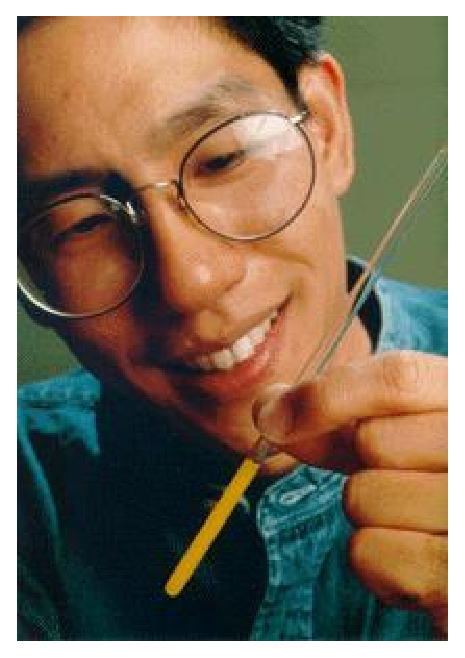
\includegraphics{20000815_chuang_vial}
\end{center}
\label{IBM'S 5 qubit quantum computer}
\caption{ Dr. Isaac Chuang, research staff member at IBM's Almaden Research Center (San Jose, Calif.), holds a quantum computer -- a glass tube containing specially designed molecules that can solve some of the most difficult mathematical problems exponentially faster than a conventional computer. }
\end{figure}


\setcounter{equation}{0}
\section{Simulation}

This project aims to produce a quantum-computer simulator that runs on classical computers. Unfortunately, any classical simulator is fundamentally inefficient compared to the quantum hardware it models. Although a quantum computer operates on a different physical paradigm than a classical computer, quantum computers cannot compute anything that classical computers cannot --- the gain is in efficiency, not in the set of computable functions. Classical machines can simulate quantum systems to arbitrary precision by storing the state-vector amplitudes and applying the unitary transformations the algorithm prescribes.

Using a classical system to simulate a quantum computer nullifies any speed advantage of the quantum algorithm: most of the structure that quantum computers exploit implicitly must be programmed and manipulated explicitly. Simulating even a moderate quantum algorithm of, say, $100$ qubits would require storing $2^{100}$ (roughly $10^{30}$) complex amplitudes --- more than any conceivable classical machine can hold, and even more far beyond what one could rotate by an arbitrary unitary in any reasonable time.

So although a quantum computer can in principle be simulated by a classical computer, the simulation becomes exponentially expensive as the qubit count grows. The memory required to store the state vector and (depending on the formulation) the operator matrices grows exponentially with the number of qubits, which is the bottleneck the parallelisation strategy of the next section is designed to push back as far as possible.

\setcounter{equation}{0}
\section{Parallel Simulation}

In this thesis, the LAM message passing interface (MPI) has been used distribute the computation (maintained by Indiana university)\footnote{http://www.lam-mpi.org/}. The program is SIMD (Single Instruction Multiple Data), with each node running a copy of the same code, but operating on different datas. The heaviest computational burden in the simulation of a quantum computer is the matrix multiplication when a register is applied a quantum program. The resulting rows of the output vector contain n multiplications, and n-1 additions for a quantum register with n qubits. Although all nodes will be running the same code, one of them will perform special tasks, it will be used to distribute the data (input vector and quantum program) and get the results (output vector). This node will be called the master node.
A strategy is to keep the probability amplitudes of each qubit on different processors, and apply the quantum gates to individual qubits. However this approach doesn't let us obtain the output vector after the execution of the quantum program, so it is required to collect the qubit's values in a single processor and perform a tensor product to get the output vector, which implies serious communication and computation overheads.
Another strategy is to assign each row of the input vector to individual nodes, and perform the computation of the corresponding row of the outcome vector on this node. Since only one row of the Quantum program is needed to calculate the output vector's row, the quantum program can be efficiently distributed. However, with this method, the nodes have to communicate the members of the input vector with each other, which increases the communication overhead, and code complexity.
Since all the nodes must have all the members of the input vector to calculate the corresponding row of the output vector, it is quite logical to distribute a copy of the input vector to all processors before execution. The program supplied with this thesis uses this strategy, it broadcasts the input vector to all nodes, to minimize the communication overhead. Then the quantum program is divided into chunks of appropriate sizes and distributed to corresponding nodes. With this strategy, it is possible to efficiently distribute the bulk of the computation among the worker nodes. After the computation is finished, the nodes begin broadcasting their results. Actually, if each node sent it's result to the master node, it would be possible to get the output vector on the master node. However, if the quantum programs are applied sequentially, this approach needs to send the output vector to the worker nodes as the input vector of the next quantum program, thus increasing the communication overhead. So it is wise to keep a copy of the output vector on all nodes to minimize the communication overhead. Depending on the network architecture, it may be more efficient to use a hypercube template to gather all the data on all the nodes (if nodes are connected with a hypercube topology). However, with a classical star topology, plain broadcasts of the results will be more efficient.

\setcounter{equation}{0}
\section{Quantum Fourier Transform}
\label{sec:qft}

The Quantum Fourier Transform (QFT) is the workhorse subroutine of quantum computing. Anywhere a quantum algorithm benefits from period finding, phase estimation, or exploitation of hidden-subgroup structure, a QFT appears. Shor's factoring algorithm is the most famous example, but the QFT also underlies Kitaev's phase estimation, the Harrow--Hassidim--Lloyd (HHL) linear-systems algorithm, and most algebraic quantum algorithms.

\subsection{Definition}

The QFT on $n$ qubits is the unitary that acts on computational-basis states as
\begin{equation}
\mathrm{QFT}\,\ket{x} \;=\; \frac{1}{\sqrt{N}}\sum_{y=0}^{N-1} e^{2\pi i\, x y / N}\,\ket{y}, \qquad N = 2^n.
\end{equation}
It is the discrete Fourier transform of the amplitude vector, applied as a unitary in $O(n^2)$ gates rather than the classical $O(N\log N)$ arithmetic operations.

\subsection{Circuit decomposition}

Write the integer $x$ in binary as $x = x_1 x_2 \ldots x_n$ (most-significant bit first). The QFT factors into a tensor product:
\begin{equation}
\mathrm{QFT}\,\ket{x_1 x_2 \ldots x_n} \;=\; \frac{1}{2^{n/2}} \bigotimes_{j=1}^{n} \Bigl(\ket{0} + e^{2\pi i\, 0.x_j x_{j+1} \ldots x_n}\,\ket{1}\Bigr),
\end{equation}
where $0.x_j x_{j+1} \ldots x_n$ denotes the binary fraction $\sum_{\ell=0}^{n-j} x_{j+\ell} \cdot 2^{-\ell-1}$. Each output qubit ends up in a single-qubit state whose relative phase depends on a suffix of the input bits.

This factorisation yields a circuit constructed from two primitives:
\begin{itemize}
\item the Hadamard gate $H = \tfrac{1}{\sqrt{2}}\bigl(\begin{smallmatrix} 1 & 1 \\ 1 & -1 \end{smallmatrix}\bigr)$;
\item controlled phase rotations $R_k = \mathrm{diag}\bigl(1, e^{2\pi i / 2^k}\bigr)$.
\end{itemize}
The structure is: for each qubit $j$ from $1$ to $n$, apply $H$ on qubit $j$, then for each later qubit $k>j$ apply a controlled-$R_{k-j+1}$ with control $k$ targeting $j$. Finish with a bit-reversal swap of all qubits, which arises because the factorisation places amplitudes in reverse bit order.

\subsection{Implementation in the simulator}

In the sparse-gate API of Section~\ref{sec:parallel}, the QFT is a short double loop:

\begin{lstlisting}[caption={QFT on $n$ qubits starting at register offset \texttt{start}.}]
void apply_qft(qreg *q, int start, int n) {
    for (int j = 0; j < n; j++) {
        int target = start + (n - 1 - j);
        apply_h(q, target);
        for (int k = j + 1; k < n; k++) {
            int control = start + (n - 1 - k);
            double theta = 2.0 * M_PI / (double)(1ULL << (k - j + 1));
            apply_controlled_phase(q, control, target, theta);
        }
    }
    /* bit-reversal swaps */
    for (int i = 0; i < n / 2; i++) {
        apply_swap(q, start + i, start + n - 1 - i);
    }
}
\end{lstlisting}

The gate count is $n$ Hadamards plus $n(n-1)/2$ controlled phases plus $n/2$ swaps, i.e., $\Theta(n^2)$ gates in total. Each gate costs $\Theta(2^n)$ work in the simulator, giving a total simulator cost of $\Theta(n^2 \cdot 2^n)$. The classical fast Fourier transform on the same $2^n$-amplitude array would cost $\Theta(n\cdot 2^n)$; the simulated QFT is therefore slower than the classical FFT by a factor of $n$. Of course, on physical quantum hardware the QFT acts on all $2^n$ amplitudes in $\Theta(n^2)$ gate time, with no enumeration of the amplitude array required, which is the whole point.

\subsection{Inverse QFT}

The inverse QFT, denoted $\mathrm{QFT}^\dagger$, is required by phase estimation (and therefore by Shor's algorithm in the next section). It is obtained by running the QFT circuit in reverse with all phase rotation angles negated. In the implementation, this means iterating the outer loop from $j = n-1$ down to $0$ and applying $R_k^\dagger$ instead of $R_k$.

\subsection{Why it matters}

The QFT is the unitary that turns periodicity into measurable phase. Given a state whose amplitudes are periodic in the basis-state index with period $r$, the QFT produces a state whose amplitudes are concentrated near multiples of $N/r$. Measuring then yields a good rational approximation to $s/r$ for some integer $s$, from which $r$ can be recovered by continued fractions. This is the eigenvalue-extracting subroutine that Shor's algorithm uses to factor integers, and that Kitaev's phase estimation uses to extract eigenvalues of arbitrary unitaries.

\setcounter{equation}{0}
\section{Grover's Algorithm}
\label{sec:grover}

\subsection{The problem}

Given a Boolean function $f:\{0,1\}^n \to \{0,1\}$ implemented as a quantum oracle, find an $x$ with $f(x)=1$. Classically, with no structure assumed on $f$, this requires $\Theta(N)$ oracle queries where $N=2^n$. Grover (1996) \cite{fqma96} showed it takes only $\Theta(\sqrt{N})$ quantum queries --- a quadratic speedup. The speedup is provably optimal for unstructured search.

\subsection{The construction}

The oracle is a \emph{phase oracle}: it applies a $-1$ phase to the marked basis states,
\begin{equation}
O_f \ket{x} \;=\; (-1)^{f(x)}\ket{x}.
\end{equation}
The bit-oracle of the previous chapter can be converted into a phase oracle using a single ancilla qubit prepared in the state $(\ket{0}-\ket{1})/\sqrt{2}$ via the standard phase-kickback trick.

Initialise the register in the uniform superposition
\begin{equation}
\ket{s} \;=\; H^{\otimes n}\ket{0\ldots 0} \;=\; \frac{1}{\sqrt{N}}\sum_{x=0}^{N-1} \ket{x}.
\end{equation}
The Grover iteration is the unitary
\begin{equation}
G \;=\; \bigl(2\ket{s}\!\bra{s} - I\bigr)\,O_f.
\end{equation}
The first factor, $2\ket{s}\!\bra{s} - I$, is the \emph{diffusion operator}: it inverts every amplitude about the mean of all amplitudes. It admits the decomposition
\begin{equation}
2\ket{s}\!\bra{s} - I \;=\; H^{\otimes n}\,\bigl(2\ket{0\ldots 0}\!\bra{0\ldots 0} - I\bigr)\,H^{\otimes n},
\end{equation}
and $2\ket{0\ldots 0}\!\bra{0\ldots 0} - I$ is a phase flip on the all-zeros component, equivalent up to global sign to a multi-controlled-$Z$ with all controls negated.

\subsection{Geometric picture}

Let $\ket{w}$ be the equal superposition of all marked basis states and $\ket{w^\perp}$ the equal superposition of all unmarked states. The initial state $\ket{s}$ lies in the two-dimensional plane spanned by $\ket{w}$ and $\ket{w^\perp}$. The oracle $O_f$ is a reflection about $\ket{w^\perp}$, and the diffusion is a reflection about $\ket{s}$. Two reflections compose into a rotation, so each Grover iteration rotates $\ket{s}$ by angle $2\theta$ in this plane, where
\begin{equation}
\sin\theta \;=\; \sqrt{M/N}
\end{equation}
and $M$ is the number of marked items. After $k$ iterations, the probability of measuring a marked state is $\sin^2\bigl((2k+1)\theta\bigr)$, maximised at
\begin{equation}
k_\mathrm{opt} \;=\; \left\lfloor \frac{\pi}{4}\sqrt{\frac{N}{M}} \right\rfloor.
\end{equation}
Too few iterations and the amplitude has not rotated all the way into the marked subspace; \emph{too many} and it rotates past it. This is one of the few quantum algorithms with a tight optimal stopping point, and stopping at $k_\mathrm{opt}$ gives a success probability close to $1$.

\subsection{Implementation in the simulator}

\begin{lstlisting}[caption={Grover's algorithm: uniform-superposition initialisation followed by $k$ iterations of oracle + diffusion.}]
typedef void (*oracle_fn)(qreg *q);   /* user-supplied phase oracle */

void apply_grover(qreg *q, int n, oracle_fn oracle, int iterations) {
    /* uniform superposition */
    for (int i = 0; i < n; i++) apply_h(q, i);

    for (int iter = 0; iter < iterations; iter++) {
        oracle(q);

        /* diffusion: H, then phase flip on |0..0>, then H */
        for (int i = 0; i < n; i++) apply_h(q, i);
        for (int i = 0; i < n; i++) apply_x(q, i);
        apply_multi_controlled_z(q, n);    /* phase flip on |1..1> */
        for (int i = 0; i < n; i++) apply_x(q, i);
        for (int i = 0; i < n; i++) apply_h(q, i);
    }
}
\end{lstlisting}

The multi-controlled-$Z$ on $n$ qubits is, in a state-vector simulator, essentially free --- one amplitude needs its sign flipped:

\begin{lstlisting}[caption={Multi-controlled-$Z$ implementation in the simulator.}]
void apply_multi_controlled_z(qreg *q, int n) {
    size_t target = (1ULL << n) - 1;   /* |1..1> */
    if (target_is_local(q, target))
        q->amp[local_index(q, target)] *= -1.0;
}
\end{lstlisting}

On physical hardware this gate is not free: it decomposes into $\Theta(n)$ Toffoli gates with $\Theta(n)$ ancillas, which is the actual cost of executing Grover's algorithm on a real machine. The simulator gets to cheat here precisely because it has direct access to the amplitude array.

\subsection{Worked example}

For $N = 2^{20}$ and a single marked item, the optimal number of iterations is $\lfloor \tfrac{\pi}{4}\sqrt{2^{20}}\rfloor = 804$. Classical search would expect on the order of $N/2 \approx 524{,}000$ queries to find it. The simulator runs all $20$ qubits in $\sim 16\,\text{MB}$ of state-vector memory --- well within a single node, no cluster needed. For larger registers, the distributed state-vector strategy of Section~\ref{sec:parallel} extends Grover simulation up to the cluster's aggregate memory ceiling.

\setcounter{equation}{0}
\section{Shor's Factoring Algorithm}
\label{sec:shor}

Shor's algorithm \cite{ptafpf94} is the most famous quantum algorithm: it factors integers in polynomial time, breaking RSA in principle. The full algorithm reduces integer factoring to a quantum subroutine for finding the multiplicative order of a random element, with the order-finding subroutine itself reducing to quantum phase estimation built on the QFT of the previous section.

\subsection{Reduction to order finding}

To factor a composite integer $N$, pick a random $a$ with $\gcd(a,N)=1$. Find the multiplicative order of $a$ modulo $N$ --- the smallest positive integer $r$ with $a^r \equiv 1 \pmod{N}$. Then:
\begin{itemize}
\item if $r$ is odd, restart with a new $a$;
\item if $a^{r/2} \equiv -1 \pmod{N}$, restart;
\item otherwise, $\gcd(a^{r/2} \pm 1,\, N)$ are non-trivial factors of $N$.
\end{itemize}
The probability of obtaining a useful $r$ is bounded below by a constant: Shor showed it is at least $1/2$ for $N$ a product of two distinct odd primes, so a constant number of random choices of $a$ suffice in expectation. The classical post-processing (gcds and the continued-fraction step below) is trivial. The hard part --- the part for which we need a quantum computer --- is finding $r$.

\subsection{Order finding via quantum phase estimation}

Define the unitary $U_a$ on $n = \lceil \log_2 N \rceil$ qubits by
\begin{equation}
U_a \ket{y} \;=\; \ket{a\,y \bmod N}.
\end{equation}
The eigenvalues of $U_a$ are $e^{2\pi i\, s / r}$ for $s = 0,1,\ldots,r-1$. Quantum phase estimation extracts a (good rational approximation to a) random one of these eigenvalues, and the continued-fraction expansion recovers the denominator $r$.

The circuit uses two registers:
\begin{itemize}
\item a \emph{counting} register of $t = 2n+1$ qubits, initialised to $\ket{0}^{\otimes t}$;
\item a \emph{target} register of $n$ qubits, initialised to $\ket{1}$.
\end{itemize}
The algorithm proceeds:
\begin{enumerate}
\item Apply $H^{\otimes t}$ to the counting register, producing the uniform superposition.
\item For each counting qubit $j = 0,1,\ldots,t-1$, apply a controlled-$U_a^{2^j}$ from counting qubit $j$ to the target register. This entangles the counting register with $\ket{a^x \bmod N}$ in the target.
\item Apply the inverse QFT (Section~\ref{sec:qft}) to the counting register.
\item Measure the counting register to obtain an integer $c \in \{0,1,\ldots,2^t-1\}$.
\item Compute $r$ from $c/2^t$ via the continued-fraction expansion.
\end{enumerate}
After step 2 the joint state is
\begin{equation}
\frac{1}{\sqrt{2^t}}\sum_{x=0}^{2^t - 1} \ket{x} \ket{a^x \bmod N}.
\end{equation}
The inverse QFT in step 3 concentrates probability mass on values of $c$ such that $c/2^t \approx s/r$ for some integer $s\in\{0,1,\ldots,r-1\}$, and the continued-fraction algorithm recovers $r$ from this rational approximation with high probability.

\subsection{The expensive subroutine: modular exponentiation}

Implementing the controlled-$U_a^{2^j}$ gates is the dominant cost of Shor's algorithm. The standard construction builds quantum ripple-carry adders, lifts those to modular addition, lifts modular addition to modular multiplication, and finally lifts modular multiplication to modular exponentiation. The most efficient known circuits use $O(n^3)$ gates and dominate the algorithm's total gate count. The Beauregard $2n+1$-qubit circuit \cite{beauregard2003} is the standard textbook construction.

In a state-vector simulator, there are two options.

\paragraph{Honest implementation.}
Build the modular exponentiation circuit from the same quantum adder primitives a physical machine would use. Useful for studying noise, gate counts, and ancilla overhead. The Beauregard circuit and its variants take this route.

\paragraph{Simulator shortcut.} Since the simulator has direct access to all amplitudes, we can update the target register's basis-state index classically for each non-zero amplitude in the counting register. The simulated quantum state is identical to the one produced by the honest circuit, but the time and ancilla costs are dramatically lower:

\begin{lstlisting}[caption={Modular exponentiation, single-process simulator shortcut. Iterates over basis states, classically computes $a^x \bmod N$, and rewrites the target register. See note below for the distributed case.}]
/* Note: this version assumes a single-process simulator: new_global may
 * fall on a different rank than idx, but local_of() here treats the
 * whole state vector as local. A distributed version must bucket the
 * (new_global, amp[idx]) pairs by destination rank, exchange them with
 * an MPI_Alltoallv, then accumulate into new_amp on each rank.       */
/* mod_pow: uint64_t mod_pow(uint64_t base, uint64_t exp, uint64_t mod); */
void apply_modular_exp(qreg *q, int counting_start, int t,
                       int target_start, int n,
                       uint64_t a, uint64_t N) {
    complex double *new_amp = calloc(q->local_size, sizeof *new_amp);
    for (size_t idx = 0; idx < q->local_size; idx++) {
        if (cabs(q->amp[idx]) < 1e-15) continue;
        size_t   global = global_index(q, idx);
        uint64_t x      = (global >> counting_start) & ((1ULL << t) - 1);
        uint64_t y      = (global >> target_start)   & ((1ULL << n) - 1);
        uint64_t y_new  = (y * mod_pow(a, x, N)) % N;
        size_t   new_global = (global
            & ~(((1ULL << n) - 1) << target_start))
            | ((size_t)y_new << target_start);
        new_amp[local_of(q, new_global)] += q->amp[idx];
    }
    memcpy(q->amp, new_amp, q->local_size * sizeof *new_amp);
    free(new_amp);
}
\end{lstlisting}

The listing as written assumes the entire state vector is held on a single process; under the distributed layout of Section~\ref{sec:parallel}, $U_a^x$ permutes basis-state indices in a way that can move amplitude across rank boundaries, so a distributed implementation must perform an all-to-all redistribution of $(\text{new\_global}, q\!\to\!\text{amp}[\text{idx}])$ pairs --- typically by bucketing per destination rank and exchanging with \verb|MPI_Alltoallv| --- before accumulating into \verb|new_amp|. This shortcut is dishonest as a model of physical execution --- it tells us nothing about real gate count or noise --- but it produces the correct quantum state for studying the information-theoretic behaviour of the algorithm, and runs in seconds where the honest circuit would take hours.

\subsection{Classical post-processing}

After measurement we have $c \in \{0, \ldots, 2^t - 1\}$. Compute the continued-fraction expansion of $c/2^t$ and find the convergent $p/q$ with $q < N$ and $|c/2^t - p/q| < 1/(2 \cdot 2^t)$. If $q$ is the true order of $a$ modulo $N$, we are done; otherwise verify $a^q \equiv 1 \pmod{N}$, and if not, restart the quantum portion of the algorithm. The continued-fraction step succeeds with constant probability per quantum run, so a constant expected number of repetitions suffices.

\subsection{Resource requirements}

To factor an $n$-bit integer $N$, Shor's algorithm requires approximately $2n+1$ counting qubits plus $n$ target qubits plus $\Theta(n)$ ancillas for modular arithmetic --- roughly $5n$ qubits in total. For RSA-2048 this is about $10{,}000$ logical qubits; under realistic surface-code overhead the physical qubit count rises to millions. This explains why factoring real-world RSA keys remains out of reach despite the algorithm being more than three decades old.

In simulation, the qubit count is the binding constraint, not the gate count, and the exact count depends on whether one simulates the \emph{honest} modular-arithmetic circuit (counting + target + arithmetic ancillas, $\approx 5n$ qubits in total) or applies a \emph{shortcut} that replaces the modular-exponentiation subcircuit with an in-place permutation of state-vector amplitudes, giving $\approx 3n+1$ qubits (counting register $t = 2n+1$ plus target register $n$, no arithmetic ancillas required). The bundled \texttt{implementation/c/}, \texttt{implementation/go/}, and \texttt{implementation/python/} libraries all use the shortcut: \texttt{apply\_modular\_exp} computes $\ket{x}\ket{y} \mapsto \ket{x}\ket{y\cdot a^x \bmod N}$ classically and then writes the result back as a single bulk permutation of the amplitude array. This is faithful to the abstract specification of the gate but is not a quantum circuit; an honest construction would unroll it into $O(n^3)$ elementary gates with $\Theta(n)$ ancillas \cite{beauregard2003}.
\begin{itemize}
\item Honest-circuit model: factoring $N=15$ ($n=4$) requires roughly $5n=20$ qubits ($16\,\text{MB}$ of state-vector memory --- fits on a phone). Factoring $N=21$ ($n=5$) requires $\sim 25$ qubits ($512\,\text{MB}$ --- fits on a laptop). Factoring a 32-bit number requires $\sim 160$ qubits, far beyond what state-vector simulation on \emph{any} conceivable classical hardware can reach.
\item Shortcut model (as bundled): factoring $N=15$ requires $3n+1 = 13$ qubits ($n=4$ target bits plus $t = 2n+1 = 9$ counting bits). Factoring $N=21$ requires $3n+1 = 16$ qubits; this is the configuration exercised by the \texttt{RUN\_SHOR\_21=1} gated test in all three implementations.
\end{itemize}
Either way, the simulation budget grows exponentially with $n$ in memory, which is the asymptotic gap that motivated the entire field --- and the reason why simulation is fundamentally a tool for algorithm design and small-scale validation, not a substitute for a physical quantum computer.

\setcounter{equation}{0}
\section{Library Documentation}

This section documents the simulator API that would replace the historical 2004 library if the sparse-gate strategy of Section~\ref{sec:parallel} were implemented in full. The 2004 source bundled with this distribution (under \texttt{implementation/\allowbreak original/}) implements the older dense-matrix approach and is preserved as a historical artifact; the API below is what the corrected design calls for.

\subsection{The quantum register}

A quantum register is represented by an opaque struct holding a local slice of the distributed state vector together with the MPI bookkeeping that identifies which slice this process owns:

\begin{lstlisting}
typedef struct {
    complex double *amp;       /* local slice of the state vector  */
    int    n_qubits;           /* total number of qubits (global)  */
    int    rank, n_procs;      /* MPI rank and process count       */
    size_t local_size;         /* 2^n_qubits / n_procs amplitudes  */
} qreg;
\end{lstlisting}

\paragraph{Construction.} \verb|qreg_create| allocates a register on the given MPI communicator and zero-initialises the amplitude array:
\begin{lstlisting}
qreg *q = qreg_create(20, MPI_COMM_WORLD);
\end{lstlisting}

\paragraph{Initialisation.} \verb|qreg_init_basis| sets the register to a definite computational basis state $\ket{k}$:
\begin{lstlisting}
qreg_init_basis(q, 0);   /* sets the register to |0...0> */
qreg_init_basis(q, 3);   /* sets it to |...011>          */
\end{lstlisting}

\paragraph{Destruction.} \verb|qreg_destroy| frees all owned memory.

\subsection{Gate primitives}

Single-qubit gates apply a $2\times 2$ unitary in place on the local amplitude slice, using the sparse-iteration pattern of Section~\ref{sec:parallel}. The library provides direct wrappers for the standard one-qubit gates and a generic primitive for user-supplied $2\times 2$ matrices:

\begin{lstlisting}
void apply_h     (qreg *q, int target);                 /* Hadamard */
void apply_x     (qreg *q, int target);                 /* Pauli-X  */
void apply_y     (qreg *q, int target);                 /* Pauli-Y  */
void apply_z     (qreg *q, int target);                 /* Pauli-Z  */
void apply_phase (qreg *q, int target, double theta);   /* diag(1,e^{i theta}) */
void apply_u     (qreg *q, int target, complex double u[2][2]);
\end{lstlisting}

Two-qubit controlled gates take a control qubit and a target qubit:
\begin{lstlisting}
void apply_cnot            (qreg *q, int control, int target);
void apply_controlled_phase(qreg *q, int control, int target, double theta);
void apply_cu              (qreg *q, int control, int target,
                            complex double u[2][2]);
void apply_swap            (qreg *q, int a, int b);
\end{lstlisting}

For each call, the library inspects whether the target/control qubits are local to this process. If both are local (the common case --- see Section~\ref{sec:parallel}) the gate is applied with no communication; otherwise the library transparently performs the pairwise amplitude exchange and then the local update.

\subsection{Measurement and inspection}

\verb|measure_all| collapses the state and returns the observed basis state on every process:
\begin{lstlisting}
size_t outcome = measure_all(q);
\end{lstlisting}

\verb|prob_of| returns $|\langle k | \psi \rangle|^2$ for a chosen basis state $k$ without disturbing the register:
\begin{lstlisting}
double p = prob_of(q, 42);
\end{lstlisting}

\verb|measure_qubit| performs a partial measurement of a single qubit and projects the state accordingly:
\begin{lstlisting}
int bit = measure_qubit(q, 3);
\end{lstlisting}

\subsection{Higher-level routines}

The chapters on the QFT (Section~\ref{sec:qft}), Grover (Section~\ref{sec:grover}), and Shor (Section~\ref{sec:shor}) build on the primitives above. The QFT is a double loop of Hadamards and controlled phases; Grover is a uniform-superposition initialisation followed by alternating oracle and diffusion calls; Shor combines phase estimation, controlled modular exponentiation, and inverse QFT. Each is exposed as a top-level function in the library so applications need not assemble the circuit by hand:

\begin{lstlisting}
void apply_qft         (qreg *q, int start, int n);
void apply_qft_inverse (qreg *q, int start, int n);
void apply_grover      (qreg *q, int n, oracle_fn oracle, int iterations);
void apply_shor_period (qreg *q, int counting_start, int t,
                        int target_start, int n,
                        int a, int N);
\end{lstlisting}

\subsection{Note on the bundled 2004 implementation}

\begin{sloppypar}
The C source under \texttt{implementation/original/} (files \texttt{matrix.c}, \texttt{parallel.c}, \texttt{qubit.c}, \texttt{standart.c}) implements a different API based on a dense \verb|matrix| struct of type \verb|__complex__ double**|:
\end{sloppypar}

\begin{lstlisting}
typedef struct {
    int row_size;
    int column_size;
    __complex__ double ** value;
} matrix;
\end{lstlisting}

with operations \verb|create_matrix|, \verb|tensor_product|, \verb|dot_product|, and the MPI primitives \verb|send_matrix|, \verb|get_matrix|, and \verb|broadcast_matrix|. This code targets the original dense-matrix strategy critiqued in Section~\ref{sec:parallel} and is retained here for historical reference. The API documented above is the design that should replace it; implementation of the corrected library is left as future work.

\setcounter{equation}{0}
\section{Conclusion}

Until quantum computers with enough qubits and low enough error rates to run useful applications become available, classical simulators will remain the primary venue for the development and analysis of quantum algorithms. The fundamental difficulty in simulating quantum systems on classical hardware --- the exponential growth of the state vector with the number of qubits --- motivates the use of parallel computation, and the simulation of small-to-medium registers across distributed clusters is a continuing area of active research.

This thesis began by introducing the four postulates of quantum mechanics, then built up the mathematical machinery (Dirac notation, the tensor product, unitary evolution, measurement) needed to describe quantum computation. It surveyed the historical landmarks of the field --- Benioff's quantum-mechanical Hamiltonian model, Feynman's quantum simulator proposal, Deutsch's quantum Turing machine, Shor's factoring algorithm, Grover's search algorithm --- and presented the three canonical algorithms in enough detail to be implementable: the Quantum Fourier Transform, Grover's unstructured search, and Shor's order-finding subroutine.

The implementation discussion was the part of the thesis that needed the most revision. The original strategy of distributing rows of a $2^n \times 2^n$ dense program matrix across MPI nodes was, as Section~\ref{sec:parallel} explains, the wrong primitive: the operator itself exceeds any conceivable memory budget for $n \gtrsim 20$, so no parallelisation strategy can rescue it. The right primitive is in-place sparse gate application directly on the state vector, with single-qubit gates costing $\Theta(2^n)$ work rather than $\Theta(2^{2n})$, and with distributed simulation arranged so that gates on low qubits cost no communication while gates on high qubits induce one pairwise exchange. The bundled 2004 C source remains as a historical record of the dense approach; a full implementation of the corrected library is left as future work.

A complete library along the lines sketched in Section~\ref{sec:parallel} and the Library Documentation chapter, with the QFT, Grover, and Shor circuits exposed as primitives, would prove useful for research into quantum algorithms --- and for teaching the subject without first requiring access to physical hardware. The Fourier transform and the algorithms that depend on it, in particular, are no longer optional features but the load-bearing core of the field.


\newpage
\addcontentsline{toc}{section}{References}
\bibliography{qucomp}

\end{document}
